\documentclass[11pt]{article}
\usepackage[margin=1in]{geometry}
\usepackage{amsmath,amssymb,amsthm,mathtools}
\usepackage{graphicx}
\usepackage{microtype}
\usepackage[hidelinks]{hyperref}
\usepackage{enumitem}
\usepackage{tikz}

\newtheorem{theorem}{Theorem}
\newtheorem{proposition}{Proposition}
\newtheorem{lemma}{Lemma}
\newcommand{\Q}{\mathbb Q}
\newcommand{\R}{\mathbb R}
\newcommand{\Z}{\mathbb Z}
\newcommand{\med}{\operatorname{med}}

\title{A Split Dedekind Cut Refutes Extension to\\
Every Proper Median Compactification}
\author{Automated mathematics run \texttt{fa\_banach\_001}, lane 7}
\date{August 11, 2026}

\begin{document}
\maketitle

\begin{center}
\fbox{\parbox{0.9\textwidth}{\textbf{Status.}
Candidate counterexample, likely valid, pending expert review.  Question 7.2
of Megrelishvili has a negative answer even for a countable rank-one median
algebra, the discrete group $\Z$, and a compact metrizable linearly ordered
median compactification.}}
\end{center}

\section{Source question and answer}

Megrelishvili proves that every continuous action by median automorphisms
extends to the minimal median compactification and then asks whether it extends
to \emph{every} proper median compactification~\cite[Question~7.2]{Intrinsic}.
In the source's notation, the question is: if $X\in(T^m_2)$ carries its
intrinsic median topology and $G\curvearrowright X$ is jointly continuous by
median automorphisms, must that action extend continuously to every proper
median compactification of $X$?

\begin{figure}[ht]
  \centering
  
\includegraphics[width=\textwidth]{figures/open_problem_crop.png}
  \caption{The source question on page 25 of arXiv:2605.16096.}
  \label{fig:question}
\end{figure}

The answer is no.  The obstruction is already visible in the elementary
theory of split linear orders: a compactification can remember two sides of
one nonprincipal cut but not the two sides of its translate.

\subsection*{Proof intuition}

The minimal completion of $\Q$ fills an irrational Dedekind cut by one point.
A different proper median compactification may split that same cut into its
left and right sides.  Translation by one carries both sides toward the single
unsplit cut one unit later.  Continuity would therefore identify the two split
points, whereas a group element must act by a homeomorphism.  The example
satisfies every hypothesis because splitting a cut outside $\Q$ neither changes
the topology induced on $\Q$ nor disturbs its order median.

\begin{theorem}\label{thm:counterexample}
There exist a median algebra $X\in(T^m_2)$ carrying its intrinsic median
topology, a jointly continuous action of a topological group $G$ by median
automorphisms, and a compact metrizable proper median compactification
$X\hookrightarrow K$ to which the action does not extend.  One may take
\[
 X=\Q,\qquad G=\Z,\qquad n\cdot q=q+n.
\]
In particular, Question 7.2 is false even for linearly ordered median
algebras.
\end{theorem}

\section{The split compactification}

Let $\overline\R=[-\infty,+\infty]$ with its usual compact order and fix
$\alpha=\sqrt2$.  Define
\[
 K=(\overline\R\setminus\{\alpha\})\cup\{\alpha^-,\alpha^+\}
\]
by leaving the order unchanged away from $\alpha$ and declaring
\[
 x<\alpha^-<\alpha^+<y
 \quad\text{whenever}\quad x<\alpha<y.
\]
Thus $\alpha^-$ and $\alpha^+$ are adjacent.  Equip $K$ with its order
topology and order median.

\begin{center}
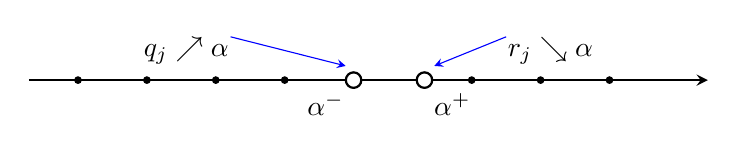
\begin{tikzpicture}[x=1.25cm,y=1cm,>=stealth]
  \draw[thick,->] (-3.3,0)--(3.6,0);
  \foreach \x in {-2.8,-2.1,-1.4,-.7,1.2,1.9,2.6}
    \fill (\x,0) circle (1.4pt);
  \filldraw[fill=white,thick] (0,0) circle (2.8pt);
  \filldraw[fill=white,thick] (.72,0) circle (2.8pt);
  \node[below left] at (0,-.05) {$\alpha^-$};
  \node[below right] at (.72,-.05) {$\alpha^+$};
  \node[above] at (-1.7,.08) {$q_j\nearrow\alpha$};
  \node[above] at (2.0,.08) {$r_j\searrow\alpha$};
  \draw[->,blue] (-1.25,.55)--(-.08,.18);
  \draw[->,blue] (1.55,.55)--(.82,.18);
\end{tikzpicture}
\end{center}

\begin{lemma}\label{lem:proper}
$K$ is a compact metrizable topological median algebra, and the natural
inclusion $\Q\hookrightarrow K$ is a dense topological median embedding.
Consequently it is a proper median compactification of
$(\Q,\tau_m)$.
\end{lemma}

\begin{proof}
The order on $K$ has first and last elements and is order complete.  Indeed,
collapse the split pair to $\alpha$.  Suprema are inherited from
$\overline\R$, with the only choice being $\alpha^-$ or $\alpha^+$ when the
projected supremum is $\alpha$; the membership of $\alpha^+$ resolves that
choice.  A complete linear order with endpoints is compact in its order
topology.  Splitting only one point preserves second countability, so $K$ is
metrizable.

Every nonempty open interval of $K$ contains a rational.  In particular,
rationals below $\alpha$ approach $\alpha^-$ and rationals above $\alpha$
approach $\alpha^+$; hence $\Q$ is dense.  Since $\alpha\notin\Q$, intersecting
an open order interval of $K$ with $\Q$ produces an ordinary open interval or
ray in $\Q$ (possibly cut at the irrational number $\alpha$).  Conversely,
ordinary rational intervals are such intersections.  Thus the subspace
topology is exactly the usual order topology on $\Q$.

The inclusion is order preserving, hence preserves the middle-of-three
median.  Finally, every LOTS is a topological median algebra: $\min$ and
$\max$ are continuous, as is immediate from inverse images of open rays, and
\[
 \med(x,y,z)=\max\{\min(x,y),\min(y,z),\min(z,x)\}.
\]
For a chain, the intrinsic median topology equals the interval topology
\cite[Proposition~4.4(1)]{Intrinsic}.  Therefore $\Q\in(T^m_2)$ and the
embedding is a proper median compactification in the exact sense of the
source.
\end{proof}

\section{Translation collapses the split pair}

\begin{proof}[Proof of Theorem~\ref{thm:counterexample}]
Give $G=\Z$ the discrete topology and let it act on $X=\Q$ by translations.
Every translation is an increasing homeomorphism and therefore a median
automorphism.  Since $G$ is discrete, the action $G\times\Q\to\Q$ is jointly
continuous.

Choose rational sequences
\[
 q_j\nearrow\alpha,\qquad r_j\searrow\alpha.
\]
In $K$ they satisfy
\[
 q_j\longrightarrow\alpha^-,\qquad
 r_j\longrightarrow\alpha^+.
\]
Suppose the action extended continuously to $K$, and denote the extension of
translation by one by $T$.  The cut $\alpha+1$ is not split in $K$, so
\[
 q_j+1\longrightarrow\alpha+1,\qquad
 r_j+1\longrightarrow\alpha+1.
\]
Continuity gives
\[
 T(\alpha^-)=\alpha+1=T(\alpha^+).
\]
Thus $T$ is not injective.  On the other hand, in any $\Z$-action the maps
corresponding to $1$ and $-1$ are mutual inverses, so $T$ must be a
homeomorphism.  This contradiction proves that no extended action exists.
\end{proof}

The MMC of $\Q$ is the ordinary Dedekind compactification
$\overline\R$, on which translations do extend.  The factor map
$K\to\overline\R$ simply collapses $\alpha^-,\alpha^+$, illustrating exactly
why minimality is compatible with the counterexample.

\section{Exact invariance criterion}

The same argument gives a useful classification.  Let $D$ be the Dedekind
compactification of a dense chain $X$, let $S$ be a set of two-sided
nonprincipal cuts, and let $K_S$ be the compact order obtained by replacing
each $s\in S$ by adjacent points $s^-<s^+$.  Write
$p:K_S\to D$ for the collapse map.

\begin{proposition}\label{prop:criterion}
Let $h$ be an increasing automorphism of $X$, and let $\widehat h$ be its
canonical extension to $D$.  Then $h$ extends to an order homeomorphism of
$K_S$ if and only if
\[
 \widehat h(S)=S.
\]
Consequently, an increasing group action on $X$ extends to $K_S$ exactly when
$S$ is invariant under the induced action on the Dedekind cuts.
\end{proposition}

\begin{proof}
Suppose $H:K_S\to K_S$ is a homeomorphism extending $h$.  The continuous maps
$pH$ and $\widehat h p$ agree on the dense copy of $X$, hence agree everywhere.
The fibers of $p$ have size two exactly over $S$.  Since $H$ is bijective and
intertwines the collapse maps, it preserves the set of two-point fibers;
therefore $\widehat h(S)=S$.

Conversely, if $\widehat h(S)=S$, define $H$ on unsplit points by
$\widehat h$ and set
\[
 H(s^-)=\widehat h(s)^-,\qquad
 H(s^+)=\widehat h(s)^+.
\]
This is an order isomorphism of compact LOTS, hence a homeomorphism, and it
extends $h$.
\end{proof}

For Theorem~\ref{thm:counterexample}, $S=\{\sqrt2\}$ is not invariant under
$q\mapsto q+1$.  Proposition~\ref{prop:criterion} shows that nonextension is
the exact orbit obstruction, rather than a sequential accident.

\section{What the cited ordered theorem actually gives}

The sentence following Question 7.2 says that the desired conclusion is true
for linearly ordered spaces and cites~\cite{Circular}.  The relevant result in
that paper assumes that the chosen proper ordered compactification already
admits extended continuous $g$-translations; it then proves that the resulting
action is jointly continuous.  The underlying ordered theorem is stated even
more explicitly in~\cite[Theorem~3.18]{Maximal}: the ordered proximity must be
$G$-invariant, or equivalently the compactification must already be a
$G_{\mathrm{discr}}$-compactification.

Thus the cited theorem is a \emph{separate-to-joint continuity} result, not an
extension-existence result for every compactification.  Proposition
\ref{prop:criterion} identifies precisely the missing hypothesis: the split
set must be invariant.  With that hypothesis restored, the ordered theorem is
fully consistent with this counterexample.

\section{Verification and review focus}

The proof is noncomputational.  It reduces to four elementary checks made
explicit above: $K$ is a compact complete order; the dense embedding induces
the intrinsic order topology on $\Q$; the middle-of-three operation is
continuous; and the two one-sided rational sequences have distinct limits
before translation but the same limit afterward.  Human review should also
compare the literal sentence after Question 7.2 with the $G$-invariance
hypothesis in~\cite[Theorem~3.18]{Maximal}.

\section{Scope and novelty}

The universal question is settled negatively by a rank-one example.  The
compactification and acting group are both metrizable/countable in the
strongest elementary sense, so no higher-rank or nonmetrizable pathology is
involved.

Local run indexes were searched by arXiv id, exact title and question, and
split-cut/translation terminology.  Bounded primary-source searches found the
source papers and standard ordered-compactification criteria but no explicit
answer to Question 7.2 or this construction.  Since split orders are classical,
novelty is asserted only relative to the specific 2026 question and remains
subject to expert review.

\begin{thebibliography}{9}
\bibitem{Intrinsic}
M. Megrelishvili,
\emph{Intrinsic uniform structure on median algebras},
arXiv:2605.16096 (2026),
\href{https://arxiv.org/abs/2605.16096}{arXiv:2605.16096}.

\bibitem{Circular}
M. Megrelishvili,
\emph{Circular orders: Topology and continuous actions},
arXiv:2512.17314 (2025),
\href{https://arxiv.org/abs/2512.17314}{arXiv:2512.17314}.

\bibitem{Maximal}
M. Megrelishvili,
\emph{Maximal equivariant compactifications},
Topology Appl. \textbf{329} (2023), 108372;
\href{https://arxiv.org/abs/2201.13426}{arXiv:2201.13426}.
\end{thebibliography}

\end{document}
